\documentclass[../../document]{subfiles}

\begin{document}
\graphicspath{{images/}}

\chapter{Theory}
\section{Electric current}
Electric current is the total charge that passes through some cross-sectional
area A per unit time. This cross-sectional area could represent a disk placed
in a gas, plasma, or liquid. \cite{practical_electronics}

If \(\Delta Q\) is the amount of charge passing through an area in a time
interval \(\Delta t\) , then the average current \(I_{\text{ave}}\) is defined as: \cite{practical_electronics}
\begin{gather}
	I_{\text{ave}} = \frac{\Delta Q}{\Delta t}.
\end{gather}

If the current changes with time, we define the instantaneous current I by
taking the limit as \(\Delta t\to 0\), so that the current is the instantaneous
rate at which charge passes through an area: \cite{practical_electronics}
\begin{gather}
	I = \lim_{\Delta t \to 0} \frac{\Delta Q}{\Delta t} = \frac{\mathrm d Q}{\mathrm d t}.
\end{gather}
The unit of current is coulombs per second, or \emph{ampere} (\(\unit{\ampere}\)):
\begin{gather}
	1\unit{\ampere} = 1\unit{\coulomb\per\second} = -6.24\times 10^{18}\unit{electrons\per\second}.
\end{gather}

\section{Voltage}
To get electrical current to flow from one point to another, a voltage must
exist between the two points. A voltage placed across a conductor gives rise to
an \emph{electromotive force} (EMF) that is responsible for giving all free
electrons within the conductor a push. \cite{practical_electronics}

Voltage is also referred to as a potential difference or just potential ---
they all mean the same thing. Volt is defined to be \cite[p. 12]{practical_electronics}
\begin{gather}
	1\unit{\volt} = \frac{1\unit{\watt}}{1\unit{\ampere}}.
\end{gather}

\section{Resistance, Resistivity, Conductivity}
In 1826, Georg Simon Ohm defined the \emph{resistance} as 
\begin{align}
	R \equiv \frac{V}{I}, && 1\unit{\ohm}=1\unit{\volt}/1\unit{\ampere}.
\end{align}
Now, Ohm’s law isn’t really a law, but rather an empirical statement about the
behavior of materials. There are some materials\footnote{That said, it only can
be applied to \emph{ohmic materials.}} for which Ohm’s law actually doesn’t
work. \cite{practical_electronics}

\paragraph*{Curious note about Ohm’s law}
Usually you see Ohm’s law written in the following form:
\begin{gather}
	V=I\times R.
\end{gather}
In this form it is tempting to define voltage in terms of resistance and
current. It is important to realize that \(R\) is the resistance of an ohmic
material and is independent of \(V\)  in Ohm’s law. Ohm’s law does not say
anything about voltage, rather, it defines resistance in terms of it and cannot
be applied to other areas of physics such as static electricity, because there
is no current flow. That’s not to say that you can’t apply Ohm’s law to, say,
predict what voltage must exist across a known resistance, given a measured
current. \cite[p. 24]{practical_electronics}

\subsection{Resistivity and Conductivity}
Resistivity is a property unique to the material. The \emph{resistivity}
\(\rho\) is defined as follows:
\begin{gather}
	\rho\equiv R\frac{A}{L},
\end{gather}
where \(A\) is a cross-sectional area, \(L\) is the wire length, \(R\) is an
overall wire resistance at provided length. It is measured in
\unit{\ohm\meter}. \cite{practical_electronics}

Conductivity is an opposite to resistivity
\begin{gather}
	\sigma\equiv \frac{1}{\rho},
\end{gather}
and is measured in siemens (\unit{1\per\ohm\meter}). \cite{practical_electronics}

Generally, within a certain temperature range, the resistivity for a large
number of metals obeys the following equation:
\begin{gather}
	\rho = \rho_0[1+\alpha(T-T_0)],
\end{gather}
where \(\rho\) is calculated resistivity based on reference resistivity
\(\rho_0\) and temperature \(T_0\). Alpha \(\alpha\) is an \emph{temperature
coefficient of resistivity} given in \unit{1\per\celsius}. \cite{practical_electronics}   

\section{Heat and Power}
Power is defined as 
\begin{gather}
	P=VI = V\frac{V}{R} = \frac{V^2}{R},\\
	P=VI=(IR)I=I^2R.
\end{gather}

\section{Resistors in circuits}
When two or more resistors are placed in \textbf{parallel}, the voltage across
each resistor is the same, but the current through each resistor will vary with
resistance. Also, the otal resistance of the combination will be lower than
that of the lowest resistance value present. \cite{practical_electronics}
\begin{gather}
	R_{\text{total}} = \frac{1}{\frac{1}{R_1}+\frac{1}{R_2}+\frac{1}{R_3}+\dots},\\
	R_{\text{total}} = \frac{R_1\times R_2}{R_1+R_2}\text{ -- two resistors in parallel}.
\end{gather}Meanwhile, current in paraller circuit is the sum of currents of every separate
component, voltage does not change:
\begin{gather}
	I_{\text{total}} = I_1+I_2+I_3+\dots+I_n,\\
	V_{\text{total}} = V_{\text{in}}.
\end{gather}

Total resistance of resistors in \textbf{series} is the sum of resistances:
\begin{gather}
	R_{\text{total}}=R_1+R_2+R_3+\dots+R_n.
\end{gather}
The sum of all the voltage drops across each series resistor will equal the
applied voltage across the combination, but current will be constant \cite{practical_electronics}
\begin{gather}
	V_{\text{total}}=V_1+V_2+V_3+\dots+V_n,\\
	I_{\text{total}} = I_{\text{const}}.
\end{gather}

\section{Voltage souces}
An \emph{ideal voltage source} is a two-terminal device that maintains a fixed
voltage across its terminals. If a variable load is connected to an ideal
voltage source, the source will maintain its terminal voltage regardless of
changes in the load resistance. This means that an ideal voltage source will
supply as much current as needed to the load in order to keep the terminal
voltage fixed. \cite{practical_electronics}
\begin{gather}
	I=\frac{V}{R},\text{ \(I\) changes with \(R\), but \(V\) is fixed}. 
\end{gather}
Now a fishy thing with an ideal voltage source is that if the resistance goes
to zero, the current must go to infinity. Well, in the real world, there is no
device that can supply an infinite amount of current. \cite{practical_electronics}

A real voltage source resembles an ideal voltage source with a small series
internal resistance or source resistance \(r_s\). This internal resistance
tends to reduce the terminal voltage, the magnitude of which depends on its
value and the amount of current that is drawn from the source. 

When a load \(R_{\text{load}}\) is attached across the source terminals,
\(R_{\text{load}}\) and \(r_s\) are connected in series. The voltage at the
terminal can be determined by using the voltage divider relation: \cite{practical_electronics}
\begin{gather}
	V_T = V_s \frac{R_{\text{load}}}{R_{\text{load}}+r_s}.
\end{gather}

An \emph{ideal current source} provides the same amount of source current \(I_s\)  at
all times to a load, regardless of load resistance changes. This means that the
terminal voltage will change as much as needed as the load resistance changes
in order to keep the source current constant. \cite{practical_electronics}

In the real world, current sources have a large internal shunt (parallel)
resistance \(r_s\). This internal resistance, which is usually very large,
tends to reduce the terminal current \(I_T\),  the magnitude of which depends
on its value and the amount of current that is drawn from the source When the
source terminals are open-circuited, \(I_T\) is zero. But when we connect a
load resistance \(R_{\text{load}}\) across source terminals,
\(R_{\text{load}}\) and \(r_s\) form and parallel resistor circuit. Using the
current divider expression, the terminal current becomes: \cite{practical_electronics}
\begin{gather}
	I_T = I_s\frac{r_s}{R_{\text{load}}+r_s}.
\end{gather}

\subsection{Combining batteries}
To \emph{increase the supply voltage}, batteries are
placed end to end or in series. The terminal voltages of each battery add together
to give a final supply voltage equal to the sum from the batteries. \cite[p. 67]{practical_electronics}

To create a \emph{supply with added current capacity} (increased operating time),
batteries can be placed in parallel--positive terminals are joined together, as
are negative terminals. \cite{practical_electronics}

\section{Kirchhoff's laws}
Kirchhoff’s laws provide the most general method for analyzing circuits. These
laws work for either linear (resistor, capacitors, and inductors) or nonlinear
elements (diodes, transistors, etc.), no matter how complex the circuit gets.
\cite{practical_electronics}
\paragraph*{Kirchhoff's voltage law}
The algebraic sum of the voltages around any loop of a circuit is zero:
\begin{gather}
	\sum_{\text{closed loop}}\Delta V = V_1+V_2+V_3+\dots+V_n = 0.
\end{gather}
In essence, Kirchhoff’s voltage law is a statement about the conservation of
energy. If an electric charge starts anywhere in a circuit and is made to go
through any loop in a circuit and back to its starting point, the net change in
its potential is zero\footnote{For example if we had closed circuit with 5\unit{\volt}
	battery and a resistor, Kirchhoff equation would be \(5\unit{\volt}-IR=0\), starting at
negative battery terminal.}. \cite{practical_electronics}
\paragraph*{Kirchhoff's current law}
The sum of the currents that enter a junction equals the sum of the currents
that leave the junction:
\begin{gather}
	\sum I_{\text{in}} = \sum I_{\text{out}}.
\end{gather}
Kirchhoff’s current law is a statement about the conservation of charge flow
through a circuit: at no time are charges created or
destroyed. \cite{practical_electronics}

\paragraph*{Superposition theorem}
The current in a branch of a linear circuit is equal to the sum of the currents
produced by each source, with the other sources set equal to zero.
\cite{practical_electronics}

The proof of the superposition theorem follows directly from the fact that
Kirchhoff’s laws applied to linear circuits always result in a set of linear
equations, which can be reduced to a single linear equation in a single
unknown. This means that an unknown branch current can thus be written as a
linear superposition of each of the source terms with an appropriate
coefficient. The superposition should not be applied to nonlinear circuits.
\cite{practical_electronics}

A source may be a voltage source or a current source. If the source is a
voltage source, to set it to zero means that the points in the circuit where
its terminals were connected must be kept at the same potential. The only way
to do this is to replace the voltage source with a conductor, creating a short
circuit. If the source is a current source, to set it to zero means to simply
remove it and leave the terminals open, thus creating an open circuit. A short
circuit causes the voltage to be zero; an open circuit causes the current to be
zero. \cite{practical_electronics}

\section{Capacitance}
Two oppositely charged parallel conducting plates separated a small distance
apart by an insulator is called a capacitor. The
ratio of charge on one of the plates of a capacitor to the voltage that exists
between the plates is called \emph{capacitance}: \cite{practical_electronics}
\begin{gather}
	C=\frac{Q}{V}
\end{gather}
C is always taken to be positive, and has units of farads (abbreviated
\(\unit{\farad}\)). \cite{practical_electronics}

\subsection{Determining capacitance}
The capacitance of a capacitor is determined by plate area \(A\) , plate
separation \(d\), and insulating material or dielectric. If a voltage \(V\)  is
applied between two parallel plates, an electric field equal to \(E = V/d\)
will be produced. From Gauss’s law, each plate must contain an equal and
opposite charge given by:
\begin{gather}
	Q=\varepsilon AE = \frac{\varepsilon AV}{d}
\end{gather}
where \(\epsilon\)  is the permittivity of the dielectric.
Free space (vacuum) has a permittivity
given by: \cite{practical_electronics}
\begin{gather}
	\varepsilon_0 = 8.85 \times 10^{-12}\unit{\farad\per\meter}
\end{gather}

The relative permittivity of a material referenced to the permittivity in
vacuum is referred to as the \emph{dielectric constant}, which is given by:
\begin{gather}
	k=\frac{\varepsilon}{\epsilon_0}.
\end{gather}
The capacitance in terms of dielectric constant is expressed as:
\begin{gather}
	C = \frac{k\varepsilon_0A}{d}.
\end{gather}
For a \emph{multiple-plate capacitor}, we use the following expression to find the
capacitance: \cite{practical_electronics}
\begin{gather}
	C = \frac{k\varepsilon_0A}{d}(n-1).
\end{gather}

\subsection{Energy in a capacitor}
The energy stored in a capacitor is found by substituting the capacitor current
into the generalized power law, then inserting the resulting power into the
definition of power, and solving for \(E\) by integration.
\cite{practical_electronics}
\begin{gather}
	E_{\text{cap}} = \frac{1}{2}CV^2.
\end{gather}
\subsection{Capacitors in parallel}
When capacitors are placed in parallel, their capacitances add, just like
resistors in series:
\begin{gather}
	C_{\text{tot}} = C_1 + C_2+\dots+C_n.
\end{gather}
It’s important to note that the largest voltage that can be applied safely to a
group of capacitors in parallel is limited to the volt- age rating of the
capacitor with the lowest voltage rating. \cite{practical_electronics}
\subsection{Capacitors in series}
When two or more capacitors are connected in series, the total capacitance is
less than that of the smallest capacitor in the group. The equivalent
capacitance is similar to resistors in parallel:
\begin{gather}
	C_{\text{tot}} = \frac{1}{C_1} + \frac{1}{C_2}+\dots+\frac{1}{C_n}.
\end{gather}
Capacitors may be connected in series to enable the group to withstand a larger
voltage than any individual capacitor is rated to withstand (the maximum
voltage ratings add). \cite{practical_electronics}

\subsection{RC Time Constant}
When a capacitor is connected to a dc voltage source, it will charge up almost
instan- taneously. Likewise, a charged capacitor that is shorted with a wire
will discharge almost instantaneously. However, with some resistance added, the
rate of charge or discharge follows an exponential pattern. There are numerous
applications that use controlled charge and discharge rates, such as timing
ICs, oscillators, waveform shapers, and low-discharge power backup
circuits. \cite{practical_electronics}

When charging a capacitor through a resistor, the voltage across the capacitor,
with respect to time, is given as:
\begin{gather}
	V(t) = V_S (1 - e^{-(t/RC)}, \tag{Charging RC}
\end{gather}
where \(V(t)\) is the capacitor voltage in volts at time \(t\) , \(V_S\) is the
source voltage, \(t\) is the time in seconds after the source voltage is
applied, \(R\)  is the circuit resistance in ohms, and \(C\) is the capacitance
in farads. Theoretically, the charging process never really finishes, but
eventually the charging current drops to an unmeasurable value. A convention
often used is to let \(t = RC\) , which makes \( V(t) = 0.632\unit{\volt}\).
The \(RC\) term is called the time constant of the circuit and is the time in
seconds required to charge the capacitor to 63.2 percent of the supply voltage.
The lowercase tau (\(\tau\)) is often used to represent \(RC\) : \(\tau = RC\).
After two time constants (\(t = 2RC = 2\tau\)), the capacitor charges ­ another
63.2 percent of the difference between the capacitor voltage at one time
constant and the supply voltage, for a total change of 86.5 percent. After
three time constants, the capacitor reaches 95 percent of the supply voltage.
After five time constants, a capacitor is considered fully charged, having
reached 99.24 percent of the source voltage. \cite{practical_electronics}

For a discharging capacitor, the following equation is used:
\cite{practical_electronics}
\begin{gather}
	V(t) = V_S e^{-(t/RC)}. \tag{Discharging RC}
\end{gather}


\subsection{Capacitors and AC}
Everything that was discussed about capacitors in dc circuits also applies in
ac circuits, with one major exception. While a capacitor in a dc circuit will
block current flow (except during brief periods of charging and discharging), a
capacitor in an ac circuit will either pass or limit current flow, depending on
frequency. Unlike a resistor that converts current energy into heat to reduce
current flow, a capacitor stores electrical energy and returns it to the
circuit. \cite{practical_electronics}

\subsection{Capacitive Reactance}
When the effect of capacitance and frequency are considered together, they
form a quantity similar to resistance. However, since no actual heat is being
generated, the effect is termed capacitive reactance. The unit for reactance
is the ohm, just as for resistors, and the formula for calculating the
reactance of a capacitor at a particular frequency is given by:
\begin{gather}
	X_C=\frac{1}{2\pi fC}=\frac{1}{\omega C} \tag{Capacitive reactance}
\end{gather} 
where \(X_C\) is an reactance in ohms, \(f\) is a frequency in \unit{\hertz}, C
is the capacitance in farads. Often omega \(\omega\) used in place of \(2\pi
f\), where \(\omega\) is called the \emph{angular frequency}.
\cite{practical_electronics}

It’s important to note that even though the unit of reactance is the ohm, there
is no power dissipated in reactance. The energy stored in the capacitor during
one portion of the cycle is simply returned to the circuit in the next. In
other words, over a complete cycle, the average power is zero.
\cite{practical_electronics}

\subsection{Capacitive divider}
\begin{wrapfigure}{l}{.3\textwidth}
	\begin{center}
		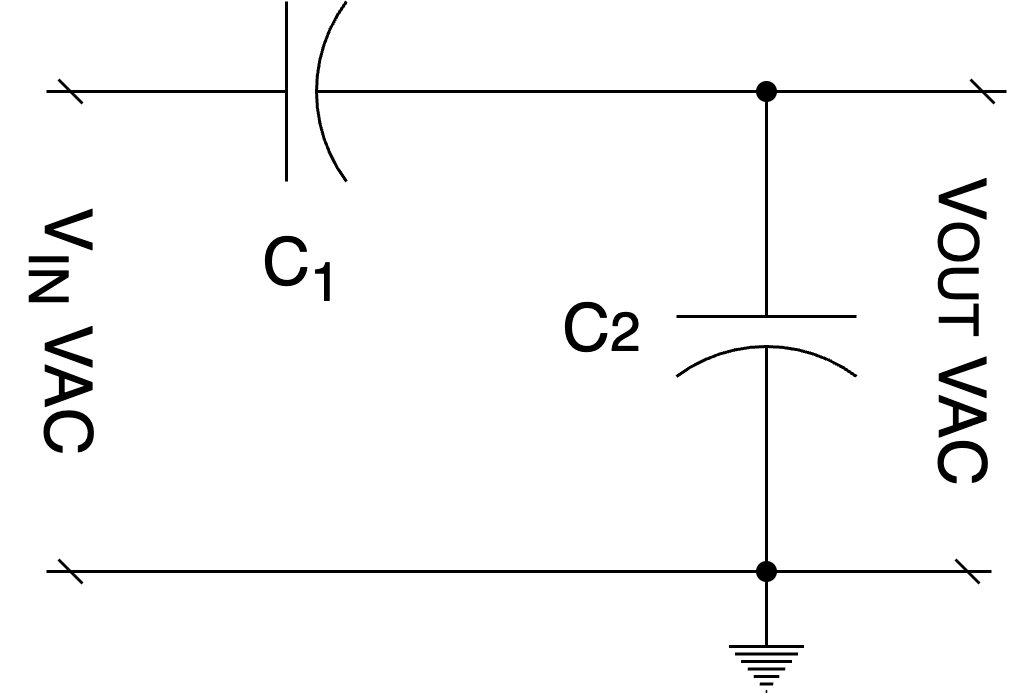
\includegraphics[width=\linewidth]{capacitive_divider.drawio.png}
	\end{center}
	\caption{Capacitive divider}\label{fig:capacitive_divider}
\end{wrapfigure}
Capacitive dividers can be used with ac input signals or even dc, since the
capacitors will rapidly reach a steady state. The formula for determining the
ac output voltage of a capacitive divider is different from the resistive
divider, because the series element, \(C_1\) is in the numerator, not \(C_2\), the
shunt element. See fig. \ref{fig:capacitive_divider}.
\begin{gather}
	V_{\text{OUT}} = \frac{C_1}{C_1+C_2}V_{\text{IN}}.
\end{gather}

Note that the output voltage is independent of the input frequency. However, if
the reactance of the capacitors is not large at the frequency of interest
(i.e., the capacitance is not large enough), the output current capability
will be very low. \cite{practical_electronics}

\subsection{Quality Factor}
Components that store energy, like a capacitor, may be compared in terms of
quality factor \(Q\), also known as the merit. The \(Q\)  of any such component
is the ratio of its ability to store energy to the sum total of all energy
losses within the component. Since reactance is associated with stored energy
and resistance is associated with energy loss, we can express the quality
factor as:
\begin{gather}
	Q=\frac{\text{Reactance}}{\text{Resistance}}=\frac{X}{R}.
\end{gather}
\(Q\)  has no units. When considering a capacitor, the reactance (in ohms) is
simply the capacitive reactance \(X=X_C\).  \(R\) is the sum of all resistances
associated with the energy losses in the component (in ohms). The \(Q\)  of
capacitors is ordinarily high. Good-quality ceramic capacitors and mica
capacitors may have \(Q\)  values of 1200 or more. Small ceramic trimmer
capacitors may have \(Q\) values too small to ignore in some applications.
Microwave capacitors can have poor \(Q\)  values, 10 or less at
10\unit{\giga\hertz} or higher. \cite{practical_electronics}

\section{Inductance}
An inductor acts like a time-varying current-sensitive resistance. It only
\enquote{resists} during changes in current; otherwise (under steady-state dc
conditions), it passes current as if it were a wire. When the applied voltage
increases, it acts like a time-dependent resistor whose resistance is greatest
during times of rapid increase in current. On the other hand, when the applied
voltage decreases, the inductor acts like a time-dependent voltage source (or
negative resistance) attempting to keep current flowing. Maximal sourcing is
greatest during times of rapid decreases in current. \cite{practical_electronics}

Amplitude of the induced voltage -- be it reverse or forward induced -- is
proportional to the rate at which the current changes, or the rate at which the
magnetic flux changes.
\begin{align}
	V_L = L\frac{\mathrm d I_L}{\mathrm dt}, && I_L = \frac{1}{L}\int V_L\mathrm d t.
\end{align}
\(L\) is called an inductance. The basic unit of inductance \(L\) is the henry,
abbreviated \unit{\henry}. One henry equals an induced voltage of 1\unit{\volt}
when the current is varying at a rate of 1\unit{\ampere\per\second}:
\cite{practical_electronics}
\begin{gather}
	1\unit{\henry} = \frac{1\unit{\volt}}{1\unit{\ampere/\second}}. \tag{Definition of a henry}
\end{gather}
Inductance of solenoid is calculated as 
\begin{gather}
	L_{\text{sol}} = \frac{\mu N^2A}{l}.
\end{gather}
Where \(\mu\) is permability of the material on which coil is wound (\(\mu
=4\pi\times 10^{7}\unit{\tesla\meter\per\ampere}\) for vacuum), \(l\) is the
length, \(A\) is the cross-sectional area of the coil, \(N\) is the number of
turns. \cite{practical_electronics}



\subsection{Self-Inductance}
Self-induction typically involves a looped wire inflicting itself with an
induced EMF that is generated by the varying current that passes through it.
According to Faraday’s law of induction, the only time that our loop can self
­inflict is when the magnetic field grows or shrinks in strength (as a result
of an increase or decrease in current). \cite{practical_electronics}

\subsection{Energy Within an Inductor}
Energy within inductor can be calculated as 
\begin{gather}
	E_L = \frac{1}{2}LI^2.
\end{gather}
Note that in a real inductor a small portion of energy is lost to resistive
heating through the inductor’s internal resistance.
\cite{practical_electronics}

\subsection{Inductorns in Series and Paraller}
When two or more inductors are connected in series, the total inductance is
equal to the sum of the individual inductances, provided the coils are
sufficiently separated, so that coils are not in the magnetic field of one
another:
\begin{gather}
	L_{\text{tot}} = L_1+L_2+L_3+\dots+L_n. \tag{Inductors in series}
\end{gather}
If inductors are connected in parallel, and if the coils are separated
sufficiently, the total inductance is given by: \cite{practical_electronics}
\begin{gather}
	\frac{1}{L_{\text{tot}}} =
	\frac{1}{L_1}+\frac{1}{L_2}+\frac{1}{L_3}+\dots+\frac{1}{L_n}. \tag{Inductors
	in parallel}
\end{gather}

\subsection{Alternating Current and Inductors}
When an alternating voltage is applied to an ideal inductance, the current that
flows through the inductor is said to lag the applied voltage by \(90^\circ\) .
Or if you like, the applied voltage leads the current by \(90^\circ\). This is
exactly the opposite of what we saw with capacitors under ac. The primary cause
for the current lag in an inductor is due to the reverse voltage generated in
the inductance. The amplitude of the reverse voltage is proportional to the
rate at which the current changes. \cite{practical_electronics}

\subsection{Inductive Reactance}
The amplitude of alternating current in an inductor is inversely proportional
to the applied frequency. Since the reverse voltage is directly proportional to
inductance for a given rate of current change, the current is inversely
proportional to inductance for a given applied voltage and frequency. The
combined effect of inductance and frequency is called inductive reactance. Like
capacitive reactance, inductive reactance is expressed in ohms. The inductive
reactance is given by the following formula:
\begin{gather}
	X_L = 2\pi fL. \tag{Inductive reactance}
\end{gather}
As \(f\)  goes to infinity, \(X_L\) goes to infinity, and the inductor acts
like an open circuit (inductors do not like to pass high-frequency signals).
However, as \(f\) goes to 0, the \(X_L\) goes to zero (inductors have an easier
time passing low-frequency signals and ideally present no \enquote{resistance}
to dc signals). \cite{practical_electronics}

\subsection{Inductive Divider}
\begin{wrapfigure}[8]{l}{.3\textwidth}
	\begin{center}
		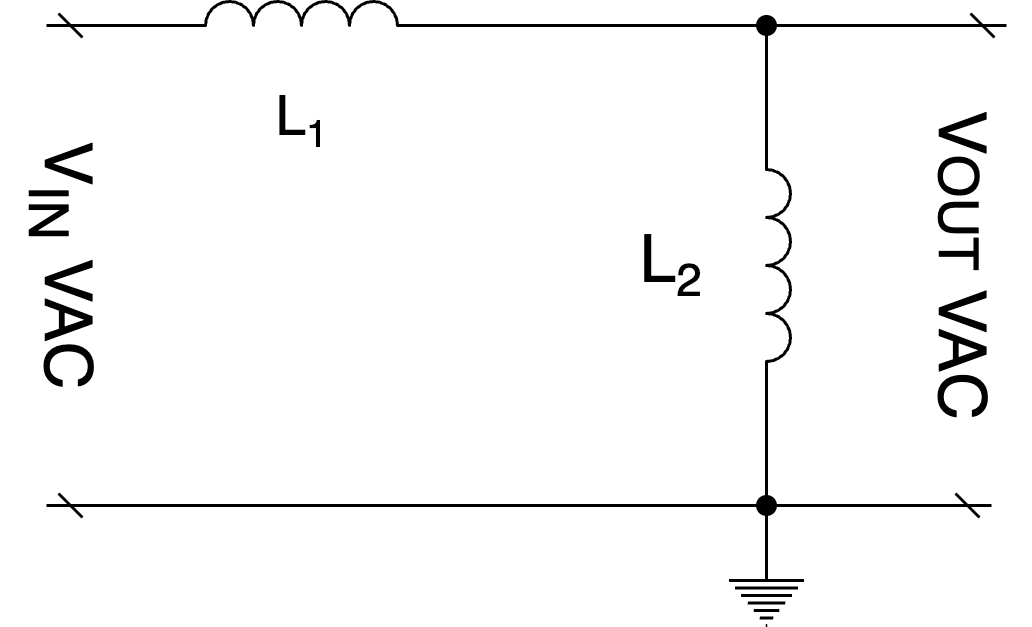
\includegraphics[width=\linewidth]{inductive_divider.drawio.png}
	\end{center}
	\caption{Inductive divider}\label{fig:inductive_divider}
\end{wrapfigure}
Inductive dividers can be used with ac input signals. A dc input voltage would
split according to the relative resistances of the two inductors by using the
resistive voltage divider. The formula for determining the ac output voltage of
an inductive divider (provided the inductors are separated -- that is, not
wound on the same core and have no mutual inductance) is: \cite{practical_electronics}
\begin{gather}
	V_{\text{out}} = \frac{L_2}{L_1+L_2}V_{\text{in}}. \tag{Inductive divider on
	fig. \ref{fig:inductive_divider}}
\end{gather}
\\

\section{Resonant Circuits}
In electrical engineering, \emph{impedance} is the opposition to alternating
current presented by the combined effect of resistance and reactance in a
circuit. \cite{slurzberg1950essentials}

When an LC circuit is driven by a sinusoidal voltage source at a special
frequency called the resonant frequency, an interesting phenomenon occurs. For
example, if you drive a series LC circuit at its resonant angular frequency
\(\omega_0 =1/LC\), or equivalently its resonant frequency \(f_0 =
1/(2\pi\sqrt{LC})\), the effective impedance across the LC network goes to
zero. In effect, the LC network acts like a short. This means that the sourced
current flow will be at a maximum. Ideally, it will go to infinity, but in
reality it is limited by internal resistances of all the components in the
circuit. \cite{practical_electronics}

Intuitively, you can imagine that the voltage across the capacitor and the
voltage across the inductor are exactly equal but opposite in phase at
resonance, within the LC series circuit. This means the effective voltage drop
across the series pair is zero; therefore, the impedance across the pair must
also be zero. \cite{practical_electronics}

Resonance occurs in a parallel LC circuit as well. The angular resonant
frequency is the same resonant frequency expression for the series LC circuit;
however, the circuit behavior is exactly opposite. Instead of the impedance
going to zero and the current going to infinity at resonance, the impedance
goes to infinity while the current goes to zero. In essence, the parallel LC
network acts like an open circuit. Of course, in reality, there is always some
internal resistance and parasitic capacitance and inductance within the circuit
that prevent this from occurring. \cite{practical_electronics}

\section{Decibels}
In electronics, often occur situations where you will need to compare the
relative amplitudes or the relative powers between two signals. If an amplifier
has an output voltage that is 10 times the input voltage (or vice-versa), ratio
can be setup:
\begin{gather}
	\frac{V_{\text{out}}}{V_{\text{in}}} = \frac{10}{1} = 10, \tag{gain}\\
	\frac{V_{\text{out}}}{V_{\text{in}}} = \frac{1}{10} = 0.1. \tag{attenuation}
\end{gather} 
A bel is defined as the logarithm of a power ratio. It gives us a
way to compare power levels with each other and with some reference power. The
bel is defined as:
\begin{gather}
	\unit{\bel} = \log\left(\frac{P_1}{P_0}\right).
\end{gather}
where \(P_0\) is the reference power and \(P_1\) is the power you are comparing
with the reference power. The more practical unit is \unit{\deci\bel}:
\cite{practical_electronics}
\begin{gather}
	\unit{\deci\bel} = 10\log\left(\frac{P_1}{P_0}\right).
\end{gather}

When \emph{doubling power}, the final power is always 2 times the initial (or
reference) power --- it ­ doesn’t make a difference if you are going from 1 to
\unit{\watt}, 40 to 80 \unit{\watt}, or 500 to 1000 \unit{\watt}, the ratio is
always 2. In decibels, a power ratio of 2 is repre sented as:
\begin{gather}
	\unit{\deci\bel} = 10\log\left(2\right) = 3.01\unit{\deci\bel}.
\end{gather}
There is a 3.01\unit{\deci\bel} gain if the output power is twice the input
power. Usually, people don’t care about the .01 fraction and simply refer to
the power doubling as a 3\unit{\deci\bel} increase in power.
\cite{practical_electronics}

When the \emph{power is cut in half}, the ratio is always 0.5. Again, it
doesn’t matter if you’re going from 1000 to 500\unit{\watt}, 80 to
40\unit{\watt}, or 2 to 1\unit{\watt}, the ratio is still 0.5. In decibels, a
power ratio of 0.5 is represented as:
\begin{gather}
	\unit{\deci\bel} = 10\log\left(0.5\right) = -3.01\unit{\deci\bel}.
\end{gather}
A negative sign indicates a decrease in power. If you increase the power by 4,
you can avoid using the decibels formula and simply associate such an increase
with doubling two times (around 6\unit{\deci\bel}).
\cite{practical_electronics}

\section{Filters}
By combining resistors, capacitors, and inductors in special ways, you can
design networks that are capable of passing certain frequencies of signals
while rejecting others. \cite[sec. 2.23]{practical_electronics}
\begin{description}
	\item[Low-Pass Filter] passes low frequencies but rejects high frequencies.
	\item[High-Pass Filter] passes high frequencies but rejects low frequencies.
	\item[Bandpass Filter] acts to pass a narrow range of frequencies while
		attenuating all other frequencies.
	\item[Notch Filter] acts to pass a wide range of frequencies, while
		attenuating a narrow band of frequencies.
\end{description}
just



\end{document}
